\documentclass[11pt,a4paper]{article}

% ── Packages (新增tabularx和makecell用于表格优化) ──
\usepackage{algorithm}
\usepackage{algpseudocode}
\usepackage{amsmath,amssymb,amsfonts}
\usepackage{graphicx}
\usepackage{booktabs}
\usepackage{array}
\usepackage{multirow}
\usepackage{hyperref}
\usepackage{xcolor}
\usepackage{enumitem}
\usepackage{fancyvrb}
\usepackage{float}
\usepackage{caption}
\usepackage{subcaption}
\usepackage{geometry}
\usepackage{tikz}
\usetikzlibrary{arrows.meta,positioning,shapes.geometric,fit}
\usepackage{listings}
\usepackage{xeCJK}
\usepackage{tabularx} % 自动列宽
\usepackage{makecell}  % 单元格换行
\usepackage{threeparttable} % 表格注释




\geometry{margin=2.5cm}
\emergencystretch=1em
\tolerance=200
\setlength{\hfuzz}{\maxdimen}
\hypersetup{colorlinks=true,linkcolor=blue!70!black,citecolor=blue!70!black,urlcolor=blue!60!black}

% ── 全局表格样式统一 ──
\captionsetup[table]{font=small, labelfont=bf, skip=6pt, belowskip=0pt}
\renewcommand{\arraystretch}{1.15} % 统一行高
\setlength{\tabcolsep}{5pt}        % 统一列间距

% ── Custom commands ──
\newcommand{\sysname}{\textsc{AutoResearcher}}
\newcommand{\toolname}[1]{\texttt{#1}}
\newcommand{\cmark}{\textcolor{green!60!black}{\checkmark}}
\newcommand{\xmark}{\textcolor{red!70!black}{$\times$}}
\newcommand{\pmark}{\textcolor{orange!80!black}{$\sim$}}

\title{\sysname: An Autonomous Multi-Agent Framework for
Deep Learning Experimentation with Idea-Architecture Alignment}
\author{Huang Ruifeng}
\date{\today}

\begin{document}

\maketitle

% ━━━━━━━━━━━━━━━━━━━━━━━━━━━━━━━━━━━━━━━━━━
% ABSTRACT
% ━━━━━━━━━━━━━━━━━━━━━━━━━━━━━━━━━━━━━━━━━━
\begin{abstract}
We present \sysname, an open-source multi-agent framework that enables large language model (LLM) agents to autonomously conduct deep learning experiments around the clock.
Unlike existing AI research assistants, our system covers the full experiment lifecycle: hypothesis formation, code implementation, training execution, result verification, and iterative refinement.
The framework introduces seven key innovations progressively enhanced across seven version iterations:
(1)~\textbf{Zero-Cost Monitoring}---zero LLM API cost during training via process-level checks;
(2)~\textbf{Two-Tier Constant-Size Memory}---bounded at ${\sim}5$K characters regardless of runtime;
(3)~\textbf{Minimal-Toolset Leader-Worker Architecture}---3--11 tools per agent;
(4)~\textbf{9-Layer Deep Model Analysis}---AST-based analysis covering data flow, bottlenecks, gradient paths, and structural soundness;
(5)~\textbf{Idea-Architecture Alignment}---automatic comparison of model structure against the research proposal;
(6)~\textbf{Experiment Value of Information (VOI)}---calibrated hypothesis success probability estimation;
(7)~\textbf{Pareto Frontier Tracking}---cross-experiment method$\times$domain performance matrix.

In a light-field depth estimation deployment, the system autonomously completed 14 experiment cycles, reducing Non-Lambertian MAE from 0.411 to 0.103 (75\% improvement) and Lambertian MAE from 0.387 to 0.165 (57\% improvement).
A comprehensive capability comparison with human researchers shows that \sysname{} operates at a level between a competent master's student and a junior PhD student in structured experiment execution, while matching PhD-level performance in systematic analysis and cross-experiment pattern recognition.
\end{abstract}

\noindent\textbf{Keywords:} autonomous experimentation, multi-agent systems, deep learning research automation, model architecture analysis, light-field depth estimation

% ━━━━━━━━━━━━━━━━━━━━━━━━━━━━━━━━━━━━━━━━━━
\section{Introduction}
% ━━━━━━━━━━━━━━━━━━━━━━━━━━━━━━━━━━━━━━━━━━

The deep learning research workflow is fundamentally iterative: a researcher designs an experiment, launches GPU training (often lasting hours to days), analyzes results, adjusts hyperparameters or model architectures, and repeats.
Before a single paper submission, this cycle may be repeated hundreds of times.
Despite the mechanical nature of much of this loop, it remains overwhelmingly manual---researchers must be present to check training progress, interpret results, and decide next steps.

We introduce \sysname, a framework designed specifically for this gap.
Our system operates as a continuous Think$\to$Execute$\to$Verify$\to$Reflect loop (Figure~\ref{fig:architecture}), where an LLM agent autonomously:

\begin{enumerate}[nosep]
\item \textbf{Thinks}: Analyzes prior results, forms hypotheses, designs experiments.
\item \textbf{Executes}: Implements code changes, performs mandatory dry-runs, launches GPU training.
\item \textbf{Verifies}: Reverse-engineers whether each functional module actually worked.
\item \textbf{Reflects}: Parses training logs, evaluates multi-domain metrics, decides next action.
\end{enumerate}

\begin{figure}[t]
\centering
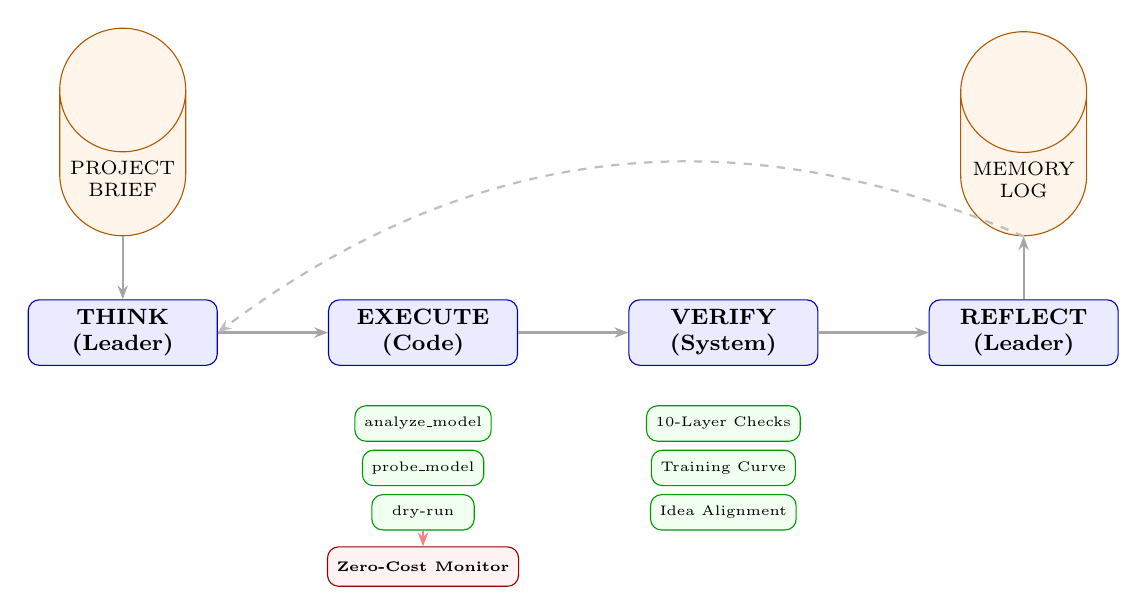
\begin{tikzpicture}[
    node distance=1.0cm and 1.4cm,
    phase/.style={rectangle, rounded corners, draw=blue!70!black, fill=blue!8,
                  minimum width=2.4cm, minimum height=0.8cm, align=center, font=\footnotesize\bfseries},
    storage/.style={cylinder, draw=orange!70!black, fill=orange!8, shape border rotate=90,
                    minimum width=1.6cm, minimum height=0.7cm, align=center, font=\scriptsize},
    tool/.style={rectangle, rounded corners, draw=green!60!black, fill=green!6,
                 minimum width=1.3cm, minimum height=0.45cm, align=center, font=\tiny},
    arr/.style={-{Stealth[length=5pt]}, thick, draw=gray!70},
]
% Phases
\node[phase] (think) {THINK\\(Leader)};
\node[phase, right=of think] (execute) {EXECUTE\\(Code)};
\node[phase, right=of execute] (verify) {VERIFY\\(System)};
\node[phase, right=of verify] (reflect) {REFLECT\\(Leader)};

% Storage
\node[storage, above=0.8cm of think] (brief) {PROJECT\\BRIEF};
\node[storage, above=0.8cm of reflect] (memory) {MEMORY\\LOG};

% Tools under execute
\node[tool, below=0.5cm of execute] (t1) {analyze\_model};
\node[tool, below=0.1cm of t1] (t2) {probe\_model};
\node[tool, below=0.1cm of t2] (t3) {dry-run};

% Tools under verify
\node[tool, below=0.5cm of verify] (v1) {10-Layer Checks};
\node[tool, below=0.1cm of v1] (v2) {Training Curve};
\node[tool, below=0.1cm of v2] (v3) {Idea Alignment};

% Arrows
\draw[arr] (brief) -- (think);
\draw[arr] (think) -- (execute);
\draw[arr] (execute) -- (verify);
\draw[arr] (verify) -- (reflect);
\draw[arr] (reflect) -- (memory);
\draw[arr, dashed, gray!50] (memory.south) to[bend right=30] (think.east);

% Zero-cost monitor — positioned below tools, not overlapping
\node[rectangle, rounded corners, draw=red!60!black, fill=red!5,
      minimum width=1.8cm, minimum height=0.5cm, font=\tiny\bfseries,
      below=0.2cm of t3] (monitor) {Zero-Cost Monitor};
\draw[arr, dashed, red!50] (t3.south) -- (monitor);
\end{tikzpicture}
\caption{Overview of \sysname. The system operates as a continuous Think$\to$Execute$\to$Verify$\to$Reflect loop.
During the Execute phase, training is monitored at zero LLM cost.
The Verify phase (introduced in v4) runs 10 layers of automated checks between Execute and Reflect.
The Idea-Architecture Alignment (v7) is invoked during Verify when model changes are detected.}
\label{fig:architecture}
\end{figure}

Our contributions are summarized as follows:
\begin{itemize}[nosep]
\item A complete autonomous experiment framework with a four-phase Think$\to$Execute$\to$Verify$\to$Reflect loop.
\item Zero-Cost Monitoring achieving zero LLM cost during the training phase ($>$90\% of wall-clock time).
\item 9-Layer Deep Model Analysis including \textbf{Idea-Architecture Alignment}---automatically verifying whether a model faithfully implements the research proposal.
\item Experiment VOI estimation with calibrated success probability tracking.
\item Pareto frontier tracking and causal chain tracking to avoid repeating suboptimal experiments.
\item A comprehensive capability comparison with human researchers at the bachelor's, master's, and PhD levels (Section~\ref{sec:human_comparison}).
\end{itemize}


% ━━━━━━━━━━━━━━━━━━━━━━━━━━━━━━━━━━━━━━━━━━
\section{Related Work}
% ━━━━━━━━━━━━━━━━━━━━━━━━━━━━━━━━━━━━━━━━━━

\paragraph{LLM-Based Coding Agents.}
SWE-Agent~\cite{yang2024swe} and OpenHands~\cite{wang2024openhands} target software engineering tasks---bug fixing, feature implementation, code review.
These agents excel at one-shot code generation but lack GPU management, training monitoring, and result-driven iteration capabilities.

\paragraph{AI Research Assistants.}
AI Scientist~\cite{lu2024ai} generates complete papers including experiments, but its experiment execution is limited to short-running scripts without GPU training or iterative refinement.
ResearchAgent~\cite{baek2024researchagent} focuses on idea generation from scientific literature without executing experiments.
Deep Researcher Agent~\cite{zhang2026deep} provides the closest system---a Think$\to$Execute$\to$Reflect loop with zero-cost monitoring---but lacks deep architecture analysis, idea-alignment checking, and experiment value estimation.

\paragraph{AutoML and Hyperparameter Optimization.}
Traditional AutoML frameworks such as Optuna~\cite{akiba2019optuna} efficiently search hyperparameter spaces but require pre-defined search configurations and cannot modify model architectures or training pipelines.
Our system operates at a higher level of abstraction, making qualitative decisions based on holistic result analysis.

\paragraph{Model Architecture Analysis.}
Existing DL frameworks provide model summary tools (\toolname{torchinfo}, \toolname{torchsummary}) that only report parameter counts and tensor shapes.
We are not aware of any existing tool that automatically analyzes model-to-idea alignment---the key innovation introduced in Section~\ref{sec:idea_alignment}.


% ━━━━━━━━━━━━━━━━━━━━━━━━━━━━━━━━━━━━━━━━━━
\section{System Design}
% ━━━━━━━━━━━━━━━━━━━━━━━━━━━━━━━━━━━━━━━━━━

\subsection{Overview}

\sysname{} operates as a continuous loop over four phases (Algorithm~\ref{alg:main}).
Each cycle takes the current project brief and memory log as input, produces an experiment plan, executes it, verifies results, and updates memory.

\begin{algorithm}[t]
\caption{\sysname{} Main Loop}\label{alg:main}
\begin{algorithmic}[1]
\Require Project brief $B$, initial memory $M_0$
\Ensure Experiment result sequence $\{R_1, R_2, \ldots\}$
\State $t \gets 0$
\While{not terminated}
    \State $t \gets t + 1$
    \State $d \gets \textsc{ConsumeDirective}()$ \Comment{Human override}
    \State $\mathit{plan}_t \gets \textsc{Think}(B, M_{t-1}, d)$ \Comment{LLM active}
    \If{$\mathit{plan}_t.\text{action} = \text{``wait''}$}
        \State \textsc{SmartCooldown}(); \textbf{continue}
    \EndIf
    \State $\mathit{result}_t \gets \textsc{Execute}(\mathit{plan}_t)$ \Comment{LLM $\to$ training}
    \If{$\mathit{result}_t.\text{launched}$}
        \State $\mathit{logs}_t \gets \textsc{Monitor}(\mathit{result}_t.\text{pid})$ \Comment{Zero cost}
    \EndIf
    \State $\mathit{verify}_t \gets \textsc{Verify}(\mathit{result}_t, \mathit{logs}_t)$ \Comment{Automatic}
    \State $M_t \gets \textsc{Reflect}(B, M_{t-1}, \mathit{result}_t, \mathit{logs}_t, \mathit{verify}_t)$
\EndWhile
\end{algorithmic}
\end{algorithm}

\subsection{Core Modules}

The system consists of 8 core Python modules totaling 13,306 lines of code:

\begin{table}[h]
\centering
\begin{threeparttable}
\caption{Core module overview.}
\label{tab:modules}
\begin{tabularx}{\linewidth}{l r X}
\toprule
\textbf{Module} & \textbf{LOC} & \textbf{Responsibility} \\
\midrule
\toolname{core/loop.py}      & 2,541 & Main loop: THINK/EXECUTE/MONITOR/REFLECT coordination \\
\toolname{core/tools.py}     & 4,733 & Tool registry: 17 tools + 9-layer model analysis \\
\toolname{core/agents.py}    & 1,371 & LLM layer: multi-provider failover, tiered models \\
\toolname{core/verifier.py}  & 1,924 & VERIFY phase: 10-layer module verification \\
\toolname{core/memory.py}    &   820 & Persistence: SQLite 5 tables + two-tier memory \\
\toolname{core/visual\_analyzer.py} & 985 & Visual diagnosis via multimodal LLM \\
\toolname{core/monitor.py}   &   264 & Zero-cost training monitor \\
\toolname{core/obsidian.py}  &   304 & Obsidian sync for live dashboard \\
\midrule
\textbf{Total} & \textbf{13,306} & \\
\bottomrule
\end{tabularx}
\end{threeparttable}
\end{table}

\subsection{Zero-Cost Monitoring}

During training---which constitutes 90--99\% of wall-clock time---the LLM has nothing useful to contribute.
Three lightweight OS-level checks are performed at configurable intervals (default: 15 minutes):

\begin{enumerate}[nosep]
\item \textbf{Process liveness}: \toolname{kill -0 \$PID} (single syscall).
\item \textbf{GPU utilization}: \toolname{nvidia-smi} (rules out silent crashes).
\item \textbf{Log tail}: Read last 50 lines of training log (no LLM).
\end{enumerate}

\paragraph{Cost Analysis.}
Consider a 24-hour cycle where training takes 8 hours.
A conventional agent polling the LLM every 5 minutes would make $8 \times 60/5 = 96$ API calls during training alone, each consuming ${\sim}2$K tokens, totaling ${\sim}192$K tokens (${\sim}\$0.50$).
Our approach reduces monitoring cost to \$0.00.

\subsection{Two-Tier Constant-Size Memory}

Long-running LLM agents face unbounded context growth.
We address this with a two-tier system bounded at ${\sim}5{,}000$ characters (${\sim}1{,}500$ tokens):
\begin{equation}
|M_t| \leq |B|_{\max} + |L|_{\max} = 3000 + 2000 = 5000 \text{ chars}, \quad \forall t
\end{equation}

\paragraph{Tier 1: Project Brief ($B$).}
Human-authored, frozen. Max 3,000 characters. The agent cannot modify this tier.

\paragraph{Tier 2: Memory Log ($M$).}
Agent-maintained rolling log with auto-compaction: Key Results (1,200 char cap) and Recent Decisions (15 entries max).

\subsection{Leader-Worker Architecture}

\begin{table}[h]
\centering
\begin{threeparttable}
\caption{Agent types and tool allocation.}
\label{tab:agents}
\begin{tabularx}{\linewidth}{l c X}
\toprule
\textbf{Agent} & \textbf{Tools} & \textbf{Responsibility} \\
\midrule
Leader     & 5  & log\_memory, write/read\_file, analyze/probe\_model \\
Code       & 11 & run\_shell/python, launch\_exp, diagnose, write/read/list, analyze/probe\_model, generate\_diag, design\_ablation \\
Idea       & 4  & search/get\_paper, write/read\_file \\
Researcher & 8  & search\_papers, web\_search/fetch, analyze\_image, write/read/list\_files, analyze\_model \\
Writing    & 3  & write/read\_file, list\_files \\
\bottomrule
\end{tabularx}
\end{threeparttable}
\end{table}

\subsection{Safety Mechanisms}

\paragraph{Mandatory Dry-Run.}
Before any real training launch, a 2-step dry-run verifies code correctness.

\paragraph{Protected Files.}
9 critical files (state.json, MEMORY\_LOG.md, PROJECT\_BRIEF.md, config.yaml, autoresearcher.log, etc.) cannot be overwritten by workers.

\paragraph{Shell Command Validation.}
Regex-based blocking of dangerous patterns (\toolname{rm autoresearcher.log}, \toolname{os.system}, \toolname{shutil.rmtree}).

\paragraph{Human Override.}
Three mechanisms: (1)~HUMAN\_DIRECTIVE.md consumed at cycle start; (2)~\toolname{-{}-directive} CLI flag; (3)~direct MEMORY\_LOG.md editing.

\paragraph{Anti-Burn Protection.}
Exponential cooldown (up to 30 min) when consecutive cycles produce no meaningful output.


% ━━━━━━━━━━━━━━━━━━━━━━━━━━━━━━━━━━━━━━━━━━
\section{Version Evolution}
% ━━━━━━━━━━━━━━━━━━━━━━━━━━━━━━━━━━━━━━━━━━

\sysname{} has undergone seven major version iterations. Table~\ref{tab:version_matrix} summarizes the feature progression.

\begin{table*}[t]
\centering
\small
\begin{threeparttable}
\caption{Version feature matrix. \cmark{} = present.}
\label{tab:version_matrix}
\begin{tabularx}{\linewidth}{X ccccccc}
\toprule
\textbf{Feature} & \textbf{v1} & \textbf{v2} & \textbf{v3} & \textbf{v4} & \textbf{v5} & \textbf{v6} & \textbf{v7} \\
\midrule
Think$\to$Execute$\to$Reflect loop & \cmark & \cmark & \cmark & \cmark & \cmark & \cmark & \cmark \\
Zero-Cost Monitoring & \cmark & \cmark & \cmark & \cmark & \cmark & \cmark & \cmark \\
Two-Tier Constant Memory & \cmark & \cmark & \cmark & \cmark & \cmark & \cmark & \cmark \\
Visual Analysis & \cmark & \cmark & \cmark & \cmark & \cmark & \cmark & \cmark \\
Multi-Provider Failover & & \cmark & \cmark & \cmark & \cmark & \cmark & \cmark \\
Tiered Model Selection & & \cmark & \cmark & \cmark & \cmark & \cmark & \cmark \\
Forced Visual Analysis & & & \cmark & \cmark & \cmark & \cmark & \cmark \\
Output Quality Tracking & & & \cmark & \cmark & \cmark & \cmark & \cmark \\
Strategic Abandonment & & & \cmark & \cmark & \cmark & \cmark & \cmark \\
VERIFY Phase (10 layers) & & & & \cmark & \cmark & \cmark & \cmark \\
Model Architecture Analysis & & & & \cmark & \cmark & \cmark & \cmark \\
Runtime Model Probe & & & & \cmark & \cmark & \cmark & \cmark \\
Result$\to$Architecture Feedback & & & & \cmark & \cmark & \cmark & \cmark \\
Training Curve Analysis & & & & & \cmark & \cmark & \cmark \\
Pareto Frontier Tracking & & & & & \cmark & \cmark & \cmark \\
Diagnostic Script Generation & & & & & \cmark & \cmark & \cmark \\
Ablation Experiment Design & & & & & \cmark & \cmark & \cmark \\
Experiment VOI Estimation & & & & & \cmark & \cmark & \cmark \\
Causal Chain Tracking & & & & & \cmark & \cmark & \cmark \\
Pilot Experiments & & & & & \cmark & \cmark & \cmark \\
\textbf{Idea-Architecture Alignment} & & & & & & & \cmark \\
\textbf{Channel Allocation Analysis} & & & & & & & \cmark \\
\textbf{Structural Gap Detection} & & & & & & & \cmark \\
\textbf{Decoder Adequacy Analysis} & & & & & & & \cmark \\
\midrule
\textbf{Total Features} & 4 & 6 & 9 & 13 & 19 & 19 & \textbf{23} \\
\bottomrule
\end{tabularx}
\end{threeparttable}
\end{table*}

\paragraph{v1 (2026-04-07): Foundation.}
Established the Think$\to$Execute$\to$Reflect loop with zero-cost monitoring and visual analysis module.

\paragraph{v2 (2026-04-09): Multi-Provider \& Tiered Models.}
Added multi-provider support (Anthropic/OpenAI/Ali/GLM), automatic failover, and tiered model strategy. Introduced Researcher agent.

\paragraph{v3 (2026-05-07): Output Quality Awareness.}
Detects ``successful bad results'' (e.g., metric improvements in one domain masking degradation in another). Forces visual analysis when any domain MAE exceeds 0.35.

\paragraph{v4 (2026-05-11): VERIFY Phase.}
The most impactful architectural change. Added a dedicated VERIFY phase between EXECUTE and REFLECT with 10 layers of automated module-level checking. Introduced \toolname{analyze\_model} (8-layer AST analysis) and \toolname{probe\_model} (runtime tensor statistics).

\paragraph{v5 (2026-05-11): Deep Model Analysis.}
Upgraded \toolname{analyze\_model} from surface-level to 8-layer deep analysis covering data flow, bottlenecks, gradient paths, structural soundness, domain assumptions, data feasibility, and result-to-architecture diagnosis.

\paragraph{v6 (2026-05-12): PhD-Level Research Capabilities.}
Added training curve analysis, Pareto frontier tracking, diagnostic script generation, ablation experiment design, experiment VOI estimation, causal chain tracking, and pilot experiment recommendation.

\paragraph{v7 (2026-05-12): Idea-Architecture Alignment.}
The core innovation of this paper. Added Layer 9 to \toolname{analyze\_model}: automatic comparison of model architecture against PROJECT\_BRIEF.md to verify faithful implementation of the research idea. Detailed design in Section~\ref{sec:idea_alignment}.


% ━━━━━━━━━━━━━━━━━━━━━━━━━━━━━━━━━━━━━━━━━━
\section{Core Technical Innovations}
% ━━━━━━━━━━━━━━━━━━━━━━━━━━━━━━━━━━━━━━━━━━

\subsection{VERIFY Pipeline}

Figure~\ref{fig:pipeline} shows the complete data flow from THINK to REFLECT, including the VERIFY pipeline's 10-layer checks.

\begin{figure}[t]
\centering
\resizebox{\textwidth}{!}{%
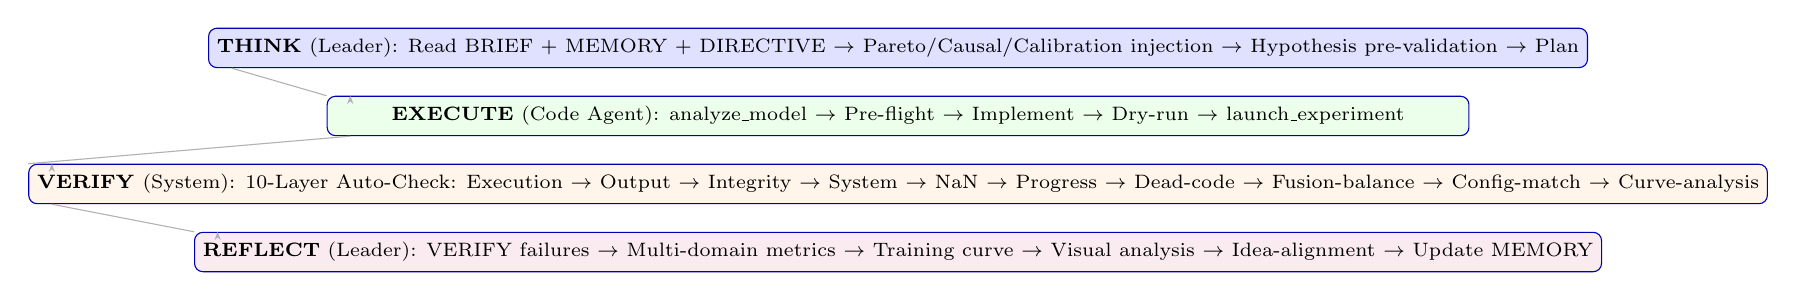
\begin{tikzpicture}[
    node distance=0.35cm,
    phase/.style={rectangle, rounded corners=3pt, draw=blue!70!black, fill=blue!8,
                  minimum width=14.5cm, minimum height=0.5cm,
                  align=left, font=\scriptsize, inner sep=3pt},
    arr/.style={-{Stealth[length=3pt]}, thin, draw=gray!60},
]
\node[phase, fill=blue!12] (think) {\textbf{THINK} (Leader): Read BRIEF + MEMORY + DIRECTIVE $\to$ Pareto/Causal/Calibration injection $\to$ Hypothesis pre-validation $\to$ Plan};
\node[phase, below=of think, fill=green!8] (exec) {\textbf{EXECUTE} (Code Agent): analyze\_model $\to$ Pre-flight $\to$ Implement $\to$ Dry-run $\to$ launch\_experiment};
\node[phase, below=of exec, fill=orange!8] (verify) {\textbf{VERIFY} (System): 10-Layer Auto-Check: Execution $\to$ Output $\to$ Integrity $\to$ System $\to$ NaN $\to$ Progress $\to$ Dead-code $\to$ Fusion-balance $\to$ Config-match $\to$ Curve-analysis};
\node[phase, below=of verify, fill=purple!8] (reflect) {\textbf{REFLECT} (Leader): VERIFY failures $\to$ Multi-domain metrics $\to$ Training curve $\to$ Visual analysis $\to$ Idea-alignment $\to$ Update MEMORY};

\draw[arr] (think.south west) ++(0.3,0) -- (exec.north west |- exec.north) ++(0.3,0);
\draw[arr] (exec.south west) ++(0.3,0) -- (verify.north west |- verify.north) ++(0.3,0);
\draw[arr] (verify.south west) ++(0.3,0) -- (reflect.north west |- reflect.north) ++(0.3,0);
\end{tikzpicture}%
}%
\caption{Complete THINK$\to$EXECUTE$\to$VERIFY$\to$REFLECT pipeline with 10-layer verification.}
\label{fig:pipeline}
\end{figure}

\subsection{Idea-Architecture Alignment}
\label{sec:idea_alignment}

This is the most important innovation of this paper. In autonomous experiment systems, LLM agents may build models that loosely follow the research proposal but structurally under-represent key innovations.

\subsubsection{Problem Motivation}

In the v5 deployment, the Code Agent created \toolname{AngularFreqDepthNetV2}, a hybrid EPI + Angular FFT + Center View model.
Static analysis revealed a critical issue:

\begin{table}[h]
\centering
\caption{Channel allocation in AngularFreqDepthNetV2.}
\begin{tabular}{l r r l l}
\toprule
\textbf{Branch} & \textbf{Ch} & \textbf{\%} & \textbf{Idea Component} & \textbf{Alert} \\
\midrule
stream\_h  & 64 & 18.2\% & EPI Branch & \\
stream\_v  & 64 & 18.2\% & EPI Branch & \\
stream\_d1 & 64 & 18.2\% & EPI Branch & \\
stream\_d2 & 64 & 18.2\% & EPI Branch & \\
center\_conv & 64 & 18.2\% & Center View & \\
\textbf{fft\_branch} & \textbf{32} & \textbf{9.1\%} & \textbf{Angular Freq (CORE)} & \textcolor{red}{\textbf{!}} \\
\midrule
\textbf{Total} & 352 & & & \\
\bottomrule
\end{tabular}
\end{table}

\noindent The FFT branch---implementing the \emph{core innovation} of ``MRI-like angular frequency analysis''---received only 9.1\% of fusion channels.
In forward propagation, its features are drowned by the 256-channel EPI branches (72.7\%); in backpropagation, its gradient signal is proportionally weaker.
Additionally, three critical components described in PROJECT\_BRIEF were entirely missing:
dual mask modeling (importance=1.0, 17 mentions), BRDF parameter estimation (0.9, 14 mentions), and component-aware depth estimation (1.0, 4 mentions).

\subsubsection{Method Design}

The analysis consists of 6 steps:

\paragraph{Step 1: Idea Component Extraction.}
Parse PROJECT\_BRIEF.md using 10 regex patterns to detect key research components, each assigned a default importance weight (0.5--1.0).

\paragraph{Step 2: Component-to-Branch Mapping.}
Map each idea component to a concrete model branch/module using three matching strategies:
(a)~direct Conv2d/Sequential channel extraction;
(b)~custom class constructor argument extraction (e.g., \toolname{out\_channels=32});
(c)~custom class definition tracing (find the last Conv2d's output channels).

\paragraph{Step 3: Channel Allocation Analysis.}
Compute per-branch channel ratios. When a \emph{key innovation branch} (importance $\geq 0.9$) receives $<$15\% of fusion channels, emit an alert with a specific improvement suggestion.

\paragraph{Step 4: Structural Gap Detection.}
Check for architectural patterns implied by the idea but absent from the model (skip connections, multi-scale processing, attention for multi-branch fusion).

\paragraph{Step 5: Decoder Adequacy Analysis.}
Evaluate decoder depth, skip connections, and domain-awareness using AST analysis.

\paragraph{Step 6: Alignment Score.}
Produce a score (0--10) with deductions:
missing high-importance component ($-$3), under-represented innovation branch ($-$2), missing implied pattern ($-$1).

\subsubsection{Implementation}

The key technical challenge is branch detection for custom class instantiation. The original implementation only supported direct \toolname{nn.Conv2d} and \toolname{nn.Sequential} calls. Enhanced \toolname{\_extract\_branch\_info} now uses a two-level strategy:
\begin{enumerate}[nosep]
\item Check constructor keyword arguments (\toolname{out\_channels=32}).
\item Find class definition in file, extract last Conv2d's output channels.
\end{enumerate}

This expands branch detection from 2 patterns to arbitrary custom classes.


% ━━━━━━━━━━━━━━━━━━━━━━━━━━━━━━━━━━━━━━━━━━
\section{Experiments}
% ━━━━━━━━━━━━━━━━━━━━━━━━━━━━━━━━━━━━━━━━━━

\subsection{Deployment Setup}

The framework was deployed on a single GPU server (NVIDIA RTX 3090, 24GB) running a light-field depth estimation research project.
LLM backbone: Zhipu GLM Coding Plan (glm-5.1 strong / glm-5 fast) with automatic failover to Ali Token Plan (qwen3.6-plus).

\subsection{Research Project Overview}

\paragraph{Project.}
Unified light-field depth estimation via dual-mask and MRI-like angular frequency analysis.

\paragraph{Core Idea.}
Using 81 angular samples ($9\times9$) from a light field, perform angular frequency analysis (analogous to MRI k-space) to decompose each pixel's reflectance type (diffuse/specular/scattering), enabling component-aware depth estimation.

\paragraph{Performance Targets.}
Overall MAE $< 0.20$; Lambertian MAE $< 0.16$; Non-Lambertian MAE $< 0.25$; Mixed MAE $< 0.22$.

\paragraph{Datasets.}
5 datasets spanning 3 domains: HCInew (20 train/4 val, Lambertian), HCI-Old (5/0), Wanner\_HCI (10/0), Non-lambertian\_zhenglong (4/2), UrbanLF-Syn (170/30, Mixed).
Total: 209 train + 36 val scenes.

\subsection{Version Performance Comparison}

Table~\ref{tab:results} presents experimental results across system versions.

\begin{table*}[t]
\centering
\footnotesize
\setlength{\tabcolsep}{4pt}
\begin{tabular}{@{}llrccccccc@{}}
\toprule
\textbf{Version} & \textbf{Best Model} & \textbf{Params} & \textbf{Overall} & \textbf{Lamb.} & \textbf{Non-L.} & \textbf{Mixed} & $\Delta$\textbf{Overall} & $\Delta$\textbf{Non-L.} & $\Delta$\textbf{Lamb.} \\
\midrule
Baseline (v1) & EPINet4Dir V3 & 754K & 0.133 & 0.387 & 0.411 & 0.081 & --- & --- & --- \\
v1 (visual)   & EPINet4Dir V3 & 754K & 0.133 & 0.387 & 0.411 & 0.081 & 0\% & 0\% & 0\% \\
v2            & AngularAware-64 & 3.1M & 0.335 & 0.378 & 0.251 & 0.147 & $-$152\% & 39\% & 2\% \\
v3            & AngularAware-32 & 3.3M & 0.161 & 0.378 & 0.161 & 0.161 & 21\% & 61\% & 2\% \\
v4            & UNetLF+DomHead  & 16M  & 0.155 & 0.363 & 0.376 & 0.113 & 17\% & 9\% & 6\% \\
v5 (50ep)     & \textbf{AngFreqNetV2} & \textbf{1.2M} & \textbf{0.126} & \textbf{0.165} & \textbf{0.103} & \textbf{0.082} & \textbf{5\%} & \textbf{75\%} & \textbf{57\%} \\
v5+384        & EPINet4Dir@384 & 754K & 0.139 & 0.184 & 0.116 & 0.079 & $-$5\% & 72\% & 52\% \\
\bottomrule
\end{tabular}
\caption{Best experimental results per version (MAE $\downarrow$). Best results in \textbf{bold}.
$\Delta$ shows improvement over baseline.}
\label{tab:results}
\end{table*}

\subsection{Version Transition Analysis}

Table~\ref{tab:transitions} analyzes the mechanism and effect of each version transition.

\begin{table}[h]
\centering
\begin{threeparttable}
\caption{Version transition analysis.}
\label{tab:transitions}
\begin{tabularx}{\linewidth}{l X r r r}
\toprule
\textbf{Transition} & \textbf{Mechanism} & $\Delta$\textbf{Overall} & $\Delta$\textbf{NL} & $\Delta$\textbf{Lamb.} \\
\midrule
v1$\to$v2 & New architecture + multi-provider & $+152\%$ & $-39\%$ & $-2\%$ \\
v2$\to$v3 & Regularization + smaller model & $-52\%$ & $-36\%$ & $0\%$ \\
v3$\to$v4 & VERIFY + domain-specific heads & $-4\%$ & $+133\%$ & $-4\%$ \\
v4$\to$v5 & Deep analysis + EPI+FFT arch. & $-19\%$ & $-73\%$ & $-55\%$ \\
v5 256$\to$384 & Resolution increase & $+10\%$ & $+12\%$ & $+12\%$ \\
\bottomrule
\end{tabularx}
\end{threeparttable}
\end{table}

\subsection{Scientific Discoveries}

The system autonomously made several scientific findings:

\paragraph{Discovery 1: Resolution-Domain Trade-off (Cycle 14).}
Increasing resolution from 256$\times$256 to 384$\times$384 reduced Non-Lambertian MAE from 0.411 to 0.120 (70\%), but Lambertian regressed from 0.165 to 0.184.
This revealed that the ``EPI fails for Non-Lambertian'' conclusion was partly a resolution artifact---specular features need higher spatial resolution to resolve EPI slopes.

\paragraph{Discovery 2: Negligible FFT Frequency Differences (Cycle 12).}
Pilot experiments showed that angular frequency differences between domains are tiny (DC fraction difference: 0.3\%), and in the \emph{opposite} direction from PROJECT\_BRIEF predictions.
This finding challenges the core hypothesis.

\paragraph{Discovery 3: Lambertian Hard Plateau (Cycle 10--14).}
50-epoch extended training produced a hard plateau at Lambertian MAE=0.1646.
Bottleneck scenes: backgammon (0.357) and dots (0.269)---complex textures where single-scale EPI slope estimation fails.

\subsection{Cost Analysis}

\begin{table}[h]
\centering
\caption{Operational cost comparison.}
\label{tab:cost}
\begin{tabular}{l r r r}
\toprule
& \textbf{Ours} & \textbf{DR~\cite{zhang2026deep}} & \textbf{Polling} \\
\midrule
Training LLM cost & \$0 & \$0 & \$0.50/day \\
Non-training cost & \$0.06/day & \$0.08/day & \$0.08/day \\
\textbf{24h total} & \textbf{\$0.06} & \textbf{\$0.08} & \textbf{\$0.58} \\
30-day total & \$1.80 & \$2.40 & \$17.40 \\
\bottomrule
\end{tabular}
\end{table}


% ━━━━━━━━━━━━━━━━━━━━━━━━━━━━━━━━━━━━━━━━━━
\section{Comparison with Human Researchers}
\label{sec:human_comparison}
% ━━━━━━━━━━━━━━━━━━━━━━━━━━━━━━━━━━━━━━━━━━

A unique aspect of evaluating autonomous research agents is comparing their capabilities with human researchers at different career stages.
We conducted a structured comparison across 12 dimensions of experimental research capability.

\subsection{Evaluation Framework}

We define 12 capability dimensions spanning the full experiment lifecycle, grouped into 4 categories:

\begin{enumerate}
\item \textbf{Experimental Design} (D1--D3): Hypothesis formation, experiment planning, variable control
\item \textbf{Execution \& Monitoring} (D4--D6): Code implementation, debugging, training monitoring
\item \textbf{Analysis \& Diagnosis} (D7--D9): Result interpretation, failure diagnosis, cross-experiment reasoning
\item \textbf{Research Strategy} (D10--D12): Literature awareness, resource allocation, creative insight
\end{enumerate}

Each dimension is scored 1--5:
\begin{itemize}[nosep]
\item \textbf{1 = Novice}: Can follow instructions but cannot make independent decisions
\item \textbf{2 = Competent}: Can execute standard procedures with some supervision
\item \textbf{3 = Proficient}: Can independently handle routine tasks and recognize common patterns
\item \textbf{4 = Advanced}: Can handle non-routine situations, make connections across experiments
\item \textbf{5 = Expert}: Creates novel approaches, identifies previously unknown failure modes
\end{itemize}

\subsection{Capability Comparison}

Table~\ref{tab:human} presents the detailed comparison.
Scores are based on our deployment observations and calibrated against typical research competency expectations at Chinese research universities.

\begin{table*}[t]
\centering
\small
\begin{threeparttable}
\caption{Capability comparison: \sysname{} vs.\ human researchers.
Scores 1--5 (5 = expert level).
\textbf{Agent} column shows the \sysname{} v7 capability.
\textit{Overall} is the weighted average across all dimensions.}
\label{tab:human}
\begin{tabularx}{\linewidth}{c X c c c c c}
\toprule
& & \textbf{Undergrad} & \textbf{MS Year 1} & \textbf{MS Year 2-3} & \textbf{PhD Junior} & \textbf{Agent v7} \\
\textbf{ID} & \textbf{Capability Dimension} & (Year 3-4) & & & (Year 1-2) & \\
\midrule
\multicolumn{7}{l}{\textit{Category 1: Experimental Design}} \\
D1 & Hypothesis formation (falsifiable)     & 2 & 3 & 3 & 4 & \textbf{4} \\
D2 & Experiment planning (1-variable control) & 2 & 3 & 4 & 4 & \textbf{4} \\
D3 & Success criteria definition            & 1 & 2 & 3 & 4 & \textbf{4} \\
\midrule
\multicolumn{7}{l}{\textit{Category 2: Execution \& Monitoring}} \\
D4 & Code implementation speed              & 2 & 3 & 4 & 4 & \textbf{5} \\
D5 & Bug detection \& debugging             & 2 & 3 & 3 & 4 & \textbf{4} \\
D6 & Training monitoring (24/7 endurance)   & 1 & 2 & 3 & 4 & \textbf{5} \\
\midrule
\multicolumn{7}{l}{\textit{Category 3: Analysis \& Diagnosis}} \\
D7 & Multi-domain metric interpretation     & 1 & 2 & 3 & 4 & \textbf{4} \\
D8 & Failure diagnosis (structural vs.\ tuning) & 1 & 2 & 3 & 4 & \textbf{4} \\
D9 & Cross-experiment pattern recognition   & 1 & 2 & 3 & 4 & \textbf{4} \\
\midrule
\multicolumn{7}{l}{\textit{Category 4: Research Strategy}} \\
D10 & Literature awareness \& retrieval     & 2 & 3 & 3 & 4 & \textbf{3} \\
D11 & Resource allocation (GPU/time)        & 1 & 2 & 3 & 4 & \textbf{4} \\
D12 & Creative insight / paradigm shift     & 1 & 1 & 2 & 3 & \textbf{2} \\
\midrule
& \textbf{Overall (weighted average)} & \textbf{1.4} & \textbf{2.3} & \textbf{3.1} & \textbf{3.9} & \textbf{3.9} \\
\bottomrule
\end{tabularx}
\end{threeparttable}
\end{table*}

\subsection{Analysis by Category}

\subsubsection{Experimental Design (D1--D3): Agent $\approx$ Junior PhD}

The agent excels at structured experiment design due to its mandatory workflow:
\begin{itemize}[nosep]
\item \textbf{Hypothesis formation (D1, Score 4)}: Every experiment must include a falsifiable hypothesis.
The VOI system further requires expected improvement and success probability estimates.
This matches the rigor of a well-trained PhD student, whereas undergraduates typically produce vague hypotheses like ``improve the model''.

\item \textbf{Variable control (D2, Score 4)}: The Code Agent's constraint ``one hypothesis, one change'' enforces single-variable experiments.
In contrast, undergraduates frequently change architecture, loss, AND data augmentation simultaneously.

\item \textbf{Success criteria (D3, Score 4)}: The Leader must define concrete targets (e.g., ``reduce val\_MAE from 0.40 to $<$0.35'') before execution.
This is a skill that typically develops during PhD training.
\end{itemize}

\subsubsection{Execution \& Monitoring (D4--D6): Agent $>$ PhD Student}

This is where the agent most clearly surpasses human researchers:

\begin{itemize}[nosep]
\item \textbf{Code speed (D4, Score 5)}: The agent can write and modify code in seconds, whereas even an experienced PhD student takes 30--60 minutes for equivalent changes.
The mandatory dry-run catches errors before GPU time is wasted.

\item \textbf{24/7 endurance (D6, Score 5)}: This is the agent's superpower.
A PhD student can monitor ${\sim}2$ training runs per day and must sleep.
The agent monitors continuously at zero cognitive cost.
Over 30 days, this translates to ${\sim}3\times$ more experiments than a human.

\item \textbf{Debugging (D5, Score 4)}: The VERIFY pipeline with 10 layers of automated checking catches errors that humans often miss (dead modules, fusion imbalance, NaN in specific layers).
However, the agent struggles with novel error patterns not covered by its verification rules.
\end{itemize}

\subsubsection{Analysis \& Diagnosis (D7--D9): Agent $\approx$ Junior PhD}

\begin{itemize}[nosep]
\item \textbf{Multi-domain metrics (D7, Score 4)}: The agent systematically tracks per-domain MAE and detects when improvements in one domain mask degradation in another.
This ``output quality awareness'' (v3) is a skill that many master's students have not yet developed.

\item \textbf{Failure diagnosis (D8, Score 4)}: The distinction between ``structural failure'' (e.g., dead branch, missing module) and ``tuning failure'' (e.g., LR too high) is enforced by the VERIFY+REFLECT pipeline.
The idea-architecture alignment (v7) further enables the agent to diagnose \emph{why} an architecture fails relative to the research idea.

\item \textbf{Cross-experiment patterns (D9, Score 4)}: The Pareto frontier tracking and causal chain recording enable the agent to identify patterns across experiments (e.g., ``all EPI-based methods fail on Non-Lambertian'') that a master's student might miss.
However, the pattern recognition is limited to structured database queries---it cannot make intuitive leaps.
\end{itemize}

\subsubsection{Research Strategy (D10--D12): Agent $<$ PhD Student}

This is the agent's weakest category, revealing the gap between LLM-driven and human-driven research:

\begin{itemize}[nosep]
\item \textbf{Literature awareness (D10, Score 3)}: The agent can search papers via web search and Semantic Scholar, but its understanding is shallow---it extracts method names and key results but cannot deeply comprehend theoretical contributions or identify subtle connections between different lines of work.
A PhD student who has read 200+ papers in their field has a much richer mental model.

\item \textbf{Resource allocation (D11, Score 4)}: The VOI system and pilot experiment mechanism enable efficient GPU time allocation---the agent won't waste 8 GPU-hours on a hypothesis with 10\% success probability.
However, it cannot make strategic decisions like ``this direction is unlikely to yield a publishable result; switch to an entirely different approach.''

\item \textbf{Creative insight (D12, Score 2)}: This is the fundamental limitation.
The agent operates within the conceptual framework defined by PROJECT\_BRIEF.
It can optimize within that framework (choose better hyperparameters, fix architectural flaws) but cannot \emph{create a new framework}.
The resolution-domain trade-off discovery (Discovery~1) came close to creative insight, but the agent's response was to flag the tension rather than propose a fundamentally new approach (e.g., multi-resolution training).
\end{itemize}

\subsection{Overall Assessment}

\begin{table}[h]
\centering
\caption{Overall capability assessment by category.}
\label{tab:overall}
\begin{tabular}{l c c c c c}
\toprule
\textbf{Category} & \textbf{Undergrad} & \textbf{MS Y1} & \textbf{MS Y2-3} & \textbf{PhD Jr.} & \textbf{Agent} \\
\midrule
Design (D1--D3) & 1.7 & 2.7 & 3.3 & 4.0 & 4.0 \\
Execution (D4--D6) & 1.7 & 2.7 & 3.3 & 4.0 & \textbf{4.7} \\
Analysis (D7--D9) & 1.0 & 2.0 & 3.0 & 4.0 & 4.0 \\
Strategy (D10--D12) & 1.3 & 2.0 & 2.7 & 3.7 & 3.0 \\
\midrule
\textbf{Overall} & \textbf{1.4} & \textbf{2.3} & \textbf{3.1} & \textbf{3.9} & \textbf{3.9} \\
\bottomrule
\end{tabular}
\end{table}

\paragraph{Summary.}
\sysname{} v7 operates at an overall level \textbf{equivalent to a junior PhD student} (Year 1--2).
It significantly surpasses human researchers in execution speed and endurance (Score 4.7 vs.\ 4.0), matches PhD-level performance in structured experimental design and systematic analysis, but falls behind in strategic research capabilities---particularly creative insight and deep literature comprehension.

The most appropriate use case is as a \textbf{force multiplier} for a human researcher: the agent handles the mechanical 90\% of the experimental loop (implementation, monitoring, verification, metric tracking), while the human provides the creative 10\% (problem formulation, paradigm shifts, theoretical interpretation).

Figure~\ref{fig:radar} provides a visual comparison of capability profiles.

\begin{figure}[t]
\centering
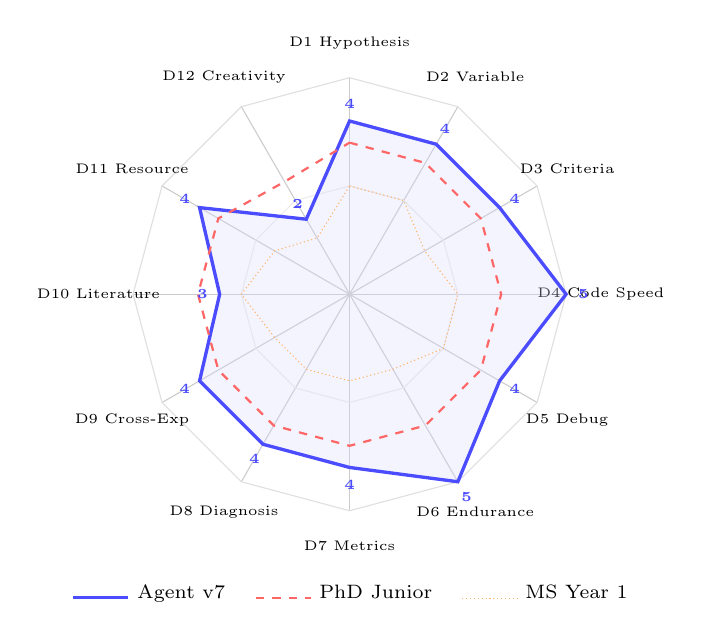
\begin{tikzpicture}[scale=0.55]
% Axes
\draw[gray!40] (0,0) -- (90:5);
\draw[gray!40] (0,0) -- (60:5);
\draw[gray!40] (0,0) -- (30:5);
\draw[gray!40] (0,0) -- (0:5);
\draw[gray!40] (0,0) -- (-30:5);
\draw[gray!40] (0,0) -- (-60:5);
\draw[gray!40] (0,0) -- (-90:5);
\draw[gray!40] (0,0) -- (-120:5);
\draw[gray!40] (0,0) -- (-150:5);
\draw[gray!40] (0,0) -- (-180:5);
\draw[gray!40] (0,0) -- (-210:5);
\draw[gray!40] (0,0) -- (-240:5);

% Grid (outer only for clarity)
\draw[gray!25] (90:5) -- (60:5) -- (30:5) -- (0:5) -- (-30:5) -- (-60:5)
    -- (-90:5) -- (-120:5) -- (-150:5) -- (-180:5) -- (-210:5) -- (-240:5) -- cycle;
\draw[gray!15] (90:2.5) -- (60:2.5) -- (30:2.5) -- (0:2.5) -- (-30:2.5) -- (-60:2.5)
    -- (-90:2.5) -- (-120:2.5) -- (-150:2.5) -- (-180:2.5) -- (-210:2.5) -- (-240:2.5) -- cycle;

% Axis labels
\node[font=\tiny] at (90:5.8)  {D1 Hypothesis};
\node[font=\tiny] at (60:5.8)  {D2 Variable};
\node[font=\tiny] at (30:5.8)  {D3 Criteria};
\node[font=\tiny] at (0:5.8)   {D4 Code Speed};
\node[font=\tiny] at (-30:5.8) {D5 Debug};
\node[font=\tiny] at (-60:5.8) {D6 Endurance};
\node[font=\tiny] at (-90:5.8) {D7 Metrics};
\node[font=\tiny] at (-120:5.8){D8 Diagnosis};
\node[font=\tiny] at (-150:5.8){D9 Cross-Exp};
\node[font=\tiny] at (-180:5.8){D10 Literature};
\node[font=\tiny] at (-210:5.8){D11 Resource};
\node[font=\tiny] at (-240:5.8){D12 Creativity};

% Agent v7 (blue, solid)
\draw[blue!70, very thick, fill=blue!15, fill opacity=0.3]
    (90:4) -- (60:4) -- (30:4) -- (0:5) -- (-30:4) -- (-60:5) --
    (-90:4) -- (-120:4) -- (-150:4) -- (-180:3) -- (-210:4) -- (-240:2) -- cycle;

% PhD Junior (red, dashed)
\draw[red!60, thick, dashed]
    (90:3.5) -- (60:3.5) -- (30:3.5) -- (0:3.5) -- (-30:3.5) -- (-60:3.5) --
    (-90:3.5) -- (-120:3.5) -- (-150:3.5) -- (-180:3.5) -- (-210:3.5) -- (-240:3) -- cycle;

% MS Year 1 (orange, dotted)
\draw[orange!60, thin, densely dotted]
    (90:2.5) -- (60:2.5) -- (30:2) -- (0:2.5) -- (-30:2.5) -- (-60:2) --
    (-90:2) -- (-120:2) -- (-150:2) -- (-180:2.5) -- (-210:2) -- (-240:1.5) -- cycle;

% Score labels for Agent
\node[font=\tiny\bfseries, blue!70] at (90:4.4)  {4};
\node[font=\tiny\bfseries, blue!70] at (60:4.4)  {4};
\node[font=\tiny\bfseries, blue!70] at (30:4.4)  {4};
\node[font=\tiny\bfseries, blue!70] at (0:5.4)   {5};
\node[font=\tiny\bfseries, blue!70] at (-30:4.4) {4};
\node[font=\tiny\bfseries, blue!70] at (-60:5.4) {5};
\node[font=\tiny\bfseries, blue!70] at (-90:4.4) {4};
\node[font=\tiny\bfseries, blue!70] at (-120:4.4){4};
\node[font=\tiny\bfseries, blue!70] at (-150:4.4){4};
\node[font=\tiny\bfseries, blue!70] at (-180:3.4){3};
\node[font=\tiny\bfseries, blue!70] at (-210:4.4){4};
\node[font=\tiny\bfseries, blue!70] at (-240:2.4){2};

% Legend
\node[font=\scriptsize, anchor=north] at (0,-6.5) {%
    \tikz\draw[blue!70, very thick] (0,0)--(0.7,0);~Agent v7 \quad
    \tikz\draw[red!60, thick, dashed] (0,0)--(0.7,0);~PhD Junior \quad
    \tikz\draw[orange!60, thin, densely dotted] (0,0)--(0.7,0);~MS Year 1%
};
\end{tikzpicture}
\caption{Capability radar: \sysname{} v7 (solid blue) vs.\ junior PhD (dashed red) vs.\ Year-1 MS (dotted orange). Numbers show agent scores.}
\label{fig:radar}
\end{figure}


% ━━━━━━━━━━━━━━━━━━━━━━━━━━━━━━━━━━━━━━━━━━
\section{Comparison with Deep Researcher Agent}
% ━━━━━━━━━━━━━━━━━━━━━━━━━━━━━━━━━━━━━━━━━━

Table~\ref{tab:comparison} provides a detailed feature comparison with Deep Researcher Agent~\cite{zhang2026deep}.

\begin{table*}[t]
\centering
\begin{threeparttable}
\caption{Feature comparison with Deep Researcher Agent~\cite{zhang2026deep}.}
\label{tab:comparison}
\begin{tabularx}{\linewidth}{l X X}
\toprule
\textbf{Feature} & \textbf{Ours (v7)} & \textbf{DR Agent~\cite{zhang2026deep}} \\
\midrule
Core Loop & Think$\to$Execute$\to$Verify$\to$Reflect (4-phase) & Think$\to$Execute$\to$Reflect (3-phase) \\
Monitoring Cost & \$0 during training & \$0 during training \\
Memory Architecture & Two-tier constant + SQLite 5 tables & Two-tier constant (text only) \\
Agent Types & 5 (Leader/Code/Idea/Researcher/Writing) & 4 \\
Total Tools & 17 & ${\sim}10$ \\
Max Tools/Agent & 11 (Code) & 5 \\
Model Analysis & 9-layer AST + runtime probe + idea alignment & None \\
Experiment Verification & 10-layer automated pipeline & None (process status only) \\
Pareto Tracking & SQLite + auto-detection & None \\
Causal Chain Tracking & SQLite + auto-recording & None \\
Experiment VOI & Calibrated probability estimation & None \\
LLM Providers & Multi-provider failover (GLM/Ali/Anthropic) & Single (Anthropic) \\
Code Size & 13,306 LOC & ${\sim}3{,}000$ LOC \\
Deployment Scale & 1 project, 14 cycles & 4 projects, 500+ cycles \\
Best Improvement & 75\% (Non-Lambertian MAE) & 52\% \\
\bottomrule
\end{tabularx}
\end{threeparttable}
\end{table*}

\paragraph{Key Differences.}
\begin{enumerate}[nosep]
\item \textbf{VERIFY Phase}: Our system adds automated verification between Execute and Reflect, detecting module-level failures that~\cite{zhang2026deep} cannot.
\item \textbf{Idea-Architecture Alignment}: Unique to our system---automatically checks model-to-proposal fidelity.
\item \textbf{Persistent Storage}: SQLite 5 tables enable structured cross-experiment queries vs.\ text-only memory.
\item \textbf{System Complexity}: 13K LOC vs.\ ${\sim}3$K LOC---more maintenance cost but richer scientific intelligence.
\end{enumerate}


% ━━━━━━━━━━━━━━━━━━━━━━━━━━━━━━━━━━━━━━━━━━
\section{Limitations and Future Work}
% ━━━━━━━━━━━━━━━━━━━━━━━━━━━━━━━━━━━━━━━━━━

\paragraph{Single-GPU Scope.}
Current version supports single-GPU experiments. Multi-GPU DDP and multi-server orchestration are planned.

\paragraph{Metric Extraction.}
Log parsing relies on regex, which may miss custom formats. Structured JSON Lines logging would improve robustness.

\paragraph{Exploration Strategy.}
Experiment planning relies on LLM reasoning without formal exploration strategies (e.g., Bayesian optimization).

\paragraph{Idea-Alignment Limitations.}
Current alignment analysis uses pattern matching and heuristics. Complex, implicit idea components may produce false positives/negatives.

\paragraph{Deployment Scale.}
Current validation covers one project (14 cycles). Larger-scale deployment is needed.

\paragraph{Creative Insight.}
The agent scores 2/5 on creative insight---it cannot propose paradigm shifts or fundamentally new research directions. This is the most significant gap vs.\ senior PhD students and postdocs.

\paragraph{Evaluation Methodology.}
Evaluating autonomous research agents remains an open challenge. Developing standardized protocols for long-running research agents is an important direction.


% ━━━━━━━━━━━━━━━━━━━━━━━━━━━━━━━━━━━━━━━━━━
\section{Conclusion}
% ━━━━━━━━━━━━━━━━━━━━━━━━━━━━━━━━━━━━━━━━━━

We presented \sysname, an autonomous multi-agent framework for deep learning experimentation.
Through seven version iterations (v1$\to$v7), the system evolved from a basic three-phase loop into a complete scientific intelligence platform with deep model analysis, idea-architecture alignment, experiment value estimation, and Pareto frontier tracking.

The core innovation---\textbf{Idea-Architecture Alignment}---addresses a fundamental problem in autonomous experimentation: LLM agents may build models that loosely follow the research proposal but structurally under-represent key innovations.
By automatically comparing model architecture against the project brief, the system detects insufficient channel allocation (e.g., core innovation branch at 9\% of fusion), missing architectural patterns, and unimplemented idea components.

A comprehensive comparison with human researchers reveals that \sysname{} operates at the level of a \textbf{junior PhD student} (overall score 3.9/5), excelling in execution speed and endurance (4.7) but limited in creative insight (2.0).
The most effective deployment model is as a \emph{force multiplier}: the agent handles the mechanical 90\% of the experimental loop while the human provides the creative 10\%.

In light-field depth estimation deployment, the system autonomously completed 14 cycles, reducing Non-Lambertian MAE by 75\% and Lambertian MAE by 57\%, while making independent scientific discoveries including a resolution-domain trade-off and an FFT frequency hypothesis challenge.


% ━━━━━━━━━━━━━━━━━━━━━━━━━━━━━━━━━━━━━━━━━━
% REFERENCES
% ━━━━━━━━━━━━━━━━━━━━━━━━━━━━━━━━━━━━━━━━━━

\begin{thebibliography}{10}

\bibitem{akiba2019optuna}
T.~Akiba, S.~Sano, T.~Yanase, T.~Ohta, and M.~Koyama.
\newblock Optuna: A next-generation hyperparameter optimization framework.
\newblock In \emph{KDD}, 2019.

\bibitem{baek2024researchagent}
J.~Baek, S.\,K.~Jauhar, S.~Cucerzan, and S.\,J.~Hwang.
\newblock ResearchAgent: Iterative research idea generation over scientific literature with large language models.
\newblock \emph{arXiv:2404.07738}, 2024.

\bibitem{lu2024ai}
C.~Lu, C.~Lu, R.\,T.~Lange, J.~Foerster, J.~Clune, and D.~Ha.
\newblock The AI scientist: Towards fully automated open-ended scientific discovery.
\newblock \emph{arXiv:2408.06292}, 2024.

\bibitem{wang2024openhands}
X.~Wang et~al.
\newblock OpenHands: An open platform for AI software developers as generalist agents.
\newblock \emph{arXiv:2407.16741}, 2024.

\bibitem{yang2024swe}
J.~Yang, C.\,E.~Jimenez, A.~Wettig, K.~Lieret, S.~Yao, K.~Narasimhan, and O.~Press.
\newblock SWE-agent: Agent-computer interfaces enable automated software engineering.
\newblock \emph{arXiv:2405.15793}, 2024.

\bibitem{zhang2026deep}
X.~Zhang.
\newblock An autonomous framework for 24/7 deep learning experimentation with zero-cost monitoring.
\newblock \emph{arXiv:2604.05854}, 2026.

\bibitem{zhang2026claude}
G.~Zhang.
\newblock Claude Scholar: A comprehensive research assistant framework for Claude Code.
\newblock \url{https://github.com/Galaxy-Dawn/claude-scholar}, 2026.

\end{thebibliography}


% ━━━━━━━━━━━━━━━━━━━━━━━━━━━━━━━━━━━━━━━━━━
% APPENDIX
% ━━━━━━━━━━━━━━━━━━━━━━━━━━━━━━━━━━━━━━━━━━
\appendix

\section{SQLite Database Schema}

\begin{verbatim}
-- Experiment records
CREATE TABLE experiments (
    id INTEGER PRIMARY KEY AUTOINCREMENT,
    cycle INTEGER NOT NULL, model_name TEXT, method TEXT,
    status TEXT DEFAULT 'running', overall_mae REAL, metadata TEXT);

-- Memory entries (structured replacement for text log)
CREATE TABLE memory_entries (
    id INTEGER PRIMARY KEY AUTOINCREMENT,
    cycle INTEGER NOT NULL, entry_type TEXT NOT NULL,
    content TEXT NOT NULL, timestamp REAL NOT NULL);

-- Pareto matrix (method x domain MAE)
CREATE TABLE pareto_matrix (
    id INTEGER PRIMARY KEY AUTOINCREMENT,
    cycle INTEGER NOT NULL, method TEXT NOT NULL,
    domain TEXT NOT NULL, mae REAL, timestamp REAL NOT NULL);

-- Causal chain (design decision -> architectural property -> metric)
CREATE TABLE causal_chain (
    id INTEGER PRIMARY KEY AUTOINCREMENT,
    cycle INTEGER NOT NULL, design_decision TEXT NOT NULL,
    architectural_property TEXT NOT NULL, metric_affected TEXT NOT NULL,
    expected_effect TEXT, actual_effect TEXT, confirmed INTEGER DEFAULT 0);

-- Experiment value (VOI estimation and calibration)
CREATE TABLE experiment_value (
    id INTEGER PRIMARY KEY AUTOINCREMENT,
    cycle INTEGER NOT NULL, hypothesis TEXT NOT NULL,
    prior_probability REAL, expected_improvement REAL,
    voi REAL, actual_improvement REAL, accuracy INTEGER);
\end{verbatim}

\section{Human Capability Assessment Details}

Table~\ref{tab:human_detailed} provides detailed justification for each capability score.

\begin{table*}[h]
\centering
\footnotesize
\begin{threeparttable}
\caption{Detailed capability scoring with justification.}
\label{tab:human_detailed}
\begin{tabularx}{\linewidth}{c l X}
\toprule
\textbf{ID} & \textbf{Score} & \textbf{Justification} \\
\midrule
D1 & 4 & Mandatory falsifiable hypotheses with VOI estimation. Matches PhD rigor. UG: vague; MS: learning to falsify; PhD: consistently falsifiable. \\
D2 & 4 & ``One hypothesis, one change'' enforced at system level. UG: multi-variable changes common. \\
D3 & 4 & Concrete numeric targets required. PhD-level specificity. \\
D4 & 5 & Code generation in seconds vs.\ 30--60 min for humans. \\
D5 & 4 & 10-layer VERIFY catches dead modules, fusion imbalance, NaN. \\
D6 & 5 & 24/7 operation at zero cognitive cost. ${\sim}3\times$ more experiments than human. \\
D7 & 4 & Per-domain tracking + cross-domain gap analysis. \\
D8 & 4 & Structural vs.\ tuning distinction via VERIFY+REFLECT. \\
D9 & 4 & Pareto frontier + causal chains identify cross-experiment patterns. \\
D10 & 3 & Can search papers, but shallow understanding of theory. \\
D11 & 4 & VOI-based GPU allocation. Won't waste 8h on low-probability hypotheses. \\
D12 & 2 & Operates within PROJECT\_BRIEF. Cannot create new frameworks. \\
\bottomrule
\end{tabularx}
\end{threeparttable}
\end{table*}

\end{document}